% Options for packages loaded elsewhere
\PassOptionsToPackage{unicode,citecolor=black}{hyperref}
\PassOptionsToPackage{hyphens}{url}
\PassOptionsToPackage{dvipsnames,svgnames,x11names}{xcolor}
%
\documentclass[
  authoryear,
  preprint,
  3p]{elsarticle}

\usepackage{amsmath,amssymb}
\usepackage{iftex}
\ifPDFTeX
  \usepackage[T1]{fontenc}
  \usepackage[utf8]{inputenc}
  \usepackage{textcomp} % provide euro and other symbols
\else % if luatex or xetex
  \usepackage{unicode-math}
  \defaultfontfeatures{Scale=MatchLowercase}
  \defaultfontfeatures[\rmfamily]{Ligatures=TeX,Scale=1}
\fi
\usepackage{lmodern}
\ifPDFTeX\else  
    % xetex/luatex font selection
\fi
% Use upquote if available, for straight quotes in verbatim environments
\IfFileExists{upquote.sty}{\usepackage{upquote}}{}
\IfFileExists{microtype.sty}{% use microtype if available
  \usepackage[]{microtype}
  \UseMicrotypeSet[protrusion]{basicmath} % disable protrusion for tt fonts
}{}
\makeatletter
\@ifundefined{KOMAClassName}{% if non-KOMA class
  \IfFileExists{parskip.sty}{%
    \usepackage{parskip}
  }{% else
    \setlength{\parindent}{0pt}
    \setlength{\parskip}{6pt plus 2pt minus 1pt}}
}{% if KOMA class
  \KOMAoptions{parskip=half}}
\makeatother
\usepackage{xcolor}
\setlength{\emergencystretch}{3em} % prevent overfull lines
\setcounter{secnumdepth}{5}
% Make \paragraph and \subparagraph free-standing
\ifx\paragraph\undefined\else
  \let\oldparagraph\paragraph
  \renewcommand{\paragraph}[1]{\oldparagraph{#1}\mbox{}}
\fi
\ifx\subparagraph\undefined\else
  \let\oldsubparagraph\subparagraph
  \renewcommand{\subparagraph}[1]{\oldsubparagraph{#1}\mbox{}}
\fi


\providecommand{\tightlist}{%
  \setlength{\itemsep}{0pt}\setlength{\parskip}{0pt}}\usepackage{longtable,booktabs,array}
\usepackage{calc} % for calculating minipage widths
% Correct order of tables after \paragraph or \subparagraph
\usepackage{etoolbox}
\makeatletter
\patchcmd\longtable{\par}{\if@noskipsec\mbox{}\fi\par}{}{}
\makeatother
% Allow footnotes in longtable head/foot
\IfFileExists{footnotehyper.sty}{\usepackage{footnotehyper}}{\usepackage{footnote}}
\makesavenoteenv{longtable}
\usepackage{graphicx}
\makeatletter
\def\maxwidth{\ifdim\Gin@nat@width>\linewidth\linewidth\else\Gin@nat@width\fi}
\def\maxheight{\ifdim\Gin@nat@height>\textheight\textheight\else\Gin@nat@height\fi}
\makeatother
% Scale images if necessary, so that they will not overflow the page
% margins by default, and it is still possible to overwrite the defaults
% using explicit options in \includegraphics[width, height, ...]{}
\setkeys{Gin}{width=\maxwidth,height=\maxheight,keepaspectratio}
% Set default figure placement to htbp
\makeatletter
\def\fps@figure{htbp}
\makeatother

\usepackage{gensymb}
\makeatletter
\makeatother
\makeatletter
\makeatother
\makeatletter
\@ifpackageloaded{caption}{}{\usepackage{caption}}
\AtBeginDocument{%
\ifdefined\contentsname
  \renewcommand*\contentsname{Table of contents}
\else
  \newcommand\contentsname{Table of contents}
\fi
\ifdefined\listfigurename
  \renewcommand*\listfigurename{List of Figures}
\else
  \newcommand\listfigurename{List of Figures}
\fi
\ifdefined\listtablename
  \renewcommand*\listtablename{List of Tables}
\else
  \newcommand\listtablename{List of Tables}
\fi
\ifdefined\figurename
  \renewcommand*\figurename{Figure}
\else
  \newcommand\figurename{Figure}
\fi
\ifdefined\tablename
  \renewcommand*\tablename{Table}
\else
  \newcommand\tablename{Table}
\fi
}
\@ifpackageloaded{float}{}{\usepackage{float}}
\floatstyle{ruled}
\@ifundefined{c@chapter}{\newfloat{codelisting}{h}{lop}}{\newfloat{codelisting}{h}{lop}[chapter]}
\floatname{codelisting}{Listing}
\newcommand*\listoflistings{\listof{codelisting}{List of Listings}}
\makeatother
\makeatletter
\@ifpackageloaded{caption}{}{\usepackage{caption}}
\@ifpackageloaded{subcaption}{}{\usepackage{subcaption}}
\makeatother
\makeatletter
\@ifpackageloaded{tcolorbox}{}{\usepackage[skins,breakable]{tcolorbox}}
\makeatother
\makeatletter
\@ifundefined{shadecolor}{\definecolor{shadecolor}{rgb}{.97, .97, .97}}
\makeatother
\makeatletter
\makeatother
\makeatletter
\makeatother
\journal{JASA-EL}
\ifLuaTeX
  \usepackage{selnolig}  % disable illegal ligatures
\fi
\usepackage[]{natbib}
\bibliographystyle{elsarticle-harv}
\IfFileExists{bookmark.sty}{\usepackage{bookmark}}{\usepackage{hyperref}}
\IfFileExists{xurl.sty}{\usepackage{xurl}}{} % add URL line breaks if available
\urlstyle{same} % disable monospaced font for URLs
\hypersetup{
  pdftitle={How to analyse and represent quantitative soundscape data},
  pdfauthor={Andrew Mitchell; Francesco Aletta; Jian Kang},
  pdfkeywords={Soundscape, Auditory Environment, ISO12913},
  colorlinks=true,
  linkcolor={blue},
  filecolor={Maroon},
  citecolor={Blue},
  urlcolor={Blue},
  pdfcreator={LaTeX via pandoc}}

\setlength{\parindent}{6pt}
\begin{document}

\begin{frontmatter}
\title{How to analyse and represent quantitative soundscape data}
\author[1]{Andrew Mitchell%
\corref{cor1}%
}
 \ead{andrew.mitchell.18@ucl.ac.uk} 
\author[1]{Francesco Aletta%
%
}
 \ead{f.aletta@ucl.ac.uk} 
\author[1]{Jian Kang%
%
}
 \ead{j.kang@ucl.ac.uk} 

\affiliation[1]{organization={University College London, Institute for
Environmental Design and Engineering},addressline={Central House, 14
Upper Woburn Place},city={London},postcode={WC1H 0NN},postcodesep={}}

\cortext[cor1]{Corresponding author}



        
\begin{abstract}
This study first examines the methods presented in ISO 12913 for
analysing and representing soundscape data by applying them to a large
existing database of soundscape assessments. The key issue identified is
the inability of the standard methods to summarise the soundscape of
locations and groups. The presented solution inherently considers the
variety of responses within a group and provides an open-source
visualisation tool to facilitate a nuanced approach to soundscape
assessment and design. Several demonstrations of the soundscape
distribution of urban spaces are presented, along with proposals for how
this approach can be used and developed.
\end{abstract}





\begin{keyword}
    Soundscape \sep Auditory Environment \sep 
    ISO12913
\end{keyword}
\end{frontmatter}
    \ifdefined\Shaded\renewenvironment{Shaded}{\begin{tcolorbox}[sharp corners, boxrule=0pt, frame hidden, interior hidden, borderline west={3pt}{0pt}{shadecolor}, enhanced, breakable]}{\end{tcolorbox}}\fi

\hypertarget{sec-introduction}{%
\section{Introduction}\label{sec-introduction}}

Methods for collecting data on how people experience acoustic
environments have been at the forefront of the debate in soundscape
studies for the past 20 years. While the soundscape research field as we
understand it today dates back to the late 1960s with the pioneering
work of authors like M. Southworth \citep{Southworth1969sonic}, R.M.
Schafer \citep{SoundscapeOursonicSchafer}, and H. Westerkamp
\citep{westerkamp2002linking}, the theme of data collection methods for
soundscape assessment emerged more prominently only recently
\citep{kang2016ten}. There is a general consensus in the research
community that standardised tools to gather and report individual
responses on the perception of urban acoustic environments are indeed
desirable, to provide comparable datasets and soundscape
characterisations across different locations, times, and samples of
people, as well as allowing for replicability studies, and offering
inputs for modelling algorithms in soundscape prediction and design
tasks. These were among the main drivers for the establishment of a
Working Group at the International Organization for Standardization
(ISO) back in 2008, which was named ``Perceptual assessment of
soundscape quality'' (ISO/TC 43/SC 1/WG 54) that has so far published
three documents within the ISO 12913 series on soundscape. Part 1 (ISO
12913-1:2014) is a full standard and provides a general framework and
definitions of soundscape concepts \citep{ISO12913_1}, while Part 2
(ISO/TS 12913-2:2018) and Part 3 (ISO/TS 12913-3:2019) are technical
specifications and offer guidance on how data should be collected and
analysed, accordingly \citep{ISO12913_2, ISO12913_3} (Part 4, on
soundscape design interventions, is currently under development by the
working group, also registered as a technical specifications document).
Specifically, Part 3 presents the proposed methods for analysing and
representing the data collected by the soundscape surveys. Since the
development of these standards, the focus has shifted from understanding
individual perception to characterising the collective perception of
increasingly large groups.

In a recent editorial paper on Soundscape Assessment, Axelsson and
colleagues observe that it is important to critically discuss current
theories and models in soundscape studies and to examine their
effectiveness, while also looking at how to integrate different methods
and perspectives for the discipline to make further advancements
\citep{Axelsson2019editorial}. This work was mainly aimed at addressing
the issue of meaningful comparability and representation of soundscape
assessments. Part 2 of the ISO 12913 standard itself does not provide
ultimate answers: the technical specifications recommend multiple
methods, as consensus around a single protocol could not be reached.
This diversity of methodological approaches should be interpreted as a
fact that soundscape theory is still under development and, for this
reason, the standardisation work should probably take a step back and
focus on developing a reference method for comparability among
soundscape studies, rather than a single protocol for soundscape data
collection. Some attempts have indeed already been made in literature
for the different methods proposed in the ISO/TS 12913-2:2018
\citep[\citet{jo2020soundscape}]{aletta2019exploring}. Neither the
standard nor the general soundscape literature has settled on effective
methods of analysing and representing the data that results from these
protocols. Data visualisations are particularly important for
understanding and communicating information as multifaceted as
soundscape perception \citep{tufte2001visual}. Although it is unlikely
that any single method will be sufficient, attempts should be made to
both facilitate future advancements in this realm and to develop a first
step approach that captures the inherent uncertainty in perception
studies, since including uncertainty is considered one of the core
principles of good data visualisation \citep{Midway2020Principles}.

This study thus aims to review the consequences of these methods for
larger datasets and provide concrete examples for how soundscapes should
be represented. In particular, we aim to strengthen the practices for
characterising the soundscape of a location, as a collective perception
by the users of the location. We also demonstrate how the progress of
these tools from their initial scope (measuring and discussing the
individual perception of a soundwalk participant) have not kept up with
recent advances and requirements for larger-scale soundscape datasets.
We question whether there are some issues related to the data collection
instruments and data analysis methods as recommended and examine the
results of the model framework and mathematical transformations laid out
in the ISO technical specifications to guide the interpretation of the
soundscape circumplex.

To examine these tools and the questions raised, we apply them to an
existing large scale, real-world dataset of soundscape assessments
collected according to the ISO methods. Finally, we propose a more
holistic and advanced method of representing soundscapes as a
probabilistic distribution of perceptions within the circumplex and
provide a toolbox for others to use.

\hypertarget{sec-current}{%
\section{The current ISO 12917 framework}\label{sec-current}}

Although different methods are proposed for data collection in ISO12913
Part 2 \citep{ISO12913_2}, in the context of this study we focus on the
questionnaire-based soundscape assessment (Method A), because it is
underpinned by a theoretical relationship among the items of the
questionnaire that compose it. The core of this questionnaire is the 8
perceptual attributes (PA) originally derived in
\citet{Axelsson2010Principal}: pleasant, vibrant (or exciting),
eventful, chaotic, annoying, monotonous, uneventful, and calm. In the
questionnaire procedure, these PAs are assessed independently of each
other, however they are conceptually considered to form a
two-dimensional circumplex with \emph{\{Pleasantness\} and
}Eventfulness* on the x- and y-axis, respectively, where all regions of
the space are equally likely to accommodate a given soundscape
assessment \citep{Aletta2016Soundscape}. In
\citet{Axelsson2010Principal}, a third primary dimension,
\emph{Familiarity} was also found, however this only accounted for 8\%
of the variance and is typically disregarded as part of the standard
circumplex. As will be made clear throughout, the circumplex model has
several aspects which make it useful for representing the soundscape
perception of a space as a whole.

\hypertarget{coordinate-transformation-into-the-two-primary-dimensions}{%
\subsection{Coordinate transformation into the two primary
dimensions}\label{coordinate-transformation-into-the-two-primary-dimensions}}

To facilitate the analysis of the PA responses, the Likert scale
responses are coded from 1 (Strongly disagree) to 5 (Strongly agree) as
ordinal variables. In order to reduce the 8 PA values into a pair of
coordinates which can be plotted on the Pleasant-Eventful axes, Part 3
of ISO 12913 \citep{ISO12913_3} provides a trigonometric transformation,
based on the \(45\degree\)-relationship between the diagonal axes and
the pleasant and eventful axes. This transformation projects the coded
values from the individual PAs down onto the primary Pleasantness and
Eventfulness dimensions then adds them together to form a single
coordinate pair. In theory, this coordinate pair then encapsulates
information from all 8 PA dimensions onto a more easily understandable
and analysable two dimensions. The ISO coordinates are thus calculated
by:

\begin{equation}\protect\hypertarget{eq-pleasant}{}{
\begin{split}
    ISO Pleasant = [(pleasant - annoying) + \cos 45\degree * (calm - chaotic) \\ + \cos 45\degree * (vibrant - monotonous)] * 1/(4+\sqrt{32)}
\end{split}
}\label{eq-pleasant}\end{equation}

\begin{equation}\protect\hypertarget{eq-eventful}{}{
\begin{split}
    ISO Eventful = [(eventful - uneventful) + \cos 45\degree * (chaotic - calm) \\ + \cos 45\degree * (vibrant - monotonous)] * 1/(4+\sqrt{32)}
\end{split}
}\label{eq-eventful}\end{equation}

where the PAs are arranged around the circumplex as shown in
Figure~\ref{fig-radar}. The \(\cos 45\degree\) term operates to project
the diagonal terms down onto the x and y axes, and the
\(1 / (4 + \sqrt{32})\) scales the resulting coordinates to the range
(-1, 1). The result of this transformation is demonstrated in
Figure~\ref{fig-radar}. This treatment of the 8 PAs makes several
assumptions and inferences about the relationships between the
dimensions. As stated in the standard \citep[5]{ISO12913_3}:

\begin{quote}
According to the two-dimensional model, vibrant soundscapes are both
pleasant and eventful, chaotic soundscapes are both eventful and
unpleasant, monotonous soundscapes are both unpleasant and uneventful,
and finally calm soundscapes are both uneventful and pleasant.
\end{quote}

\begin{figure}

{\centering 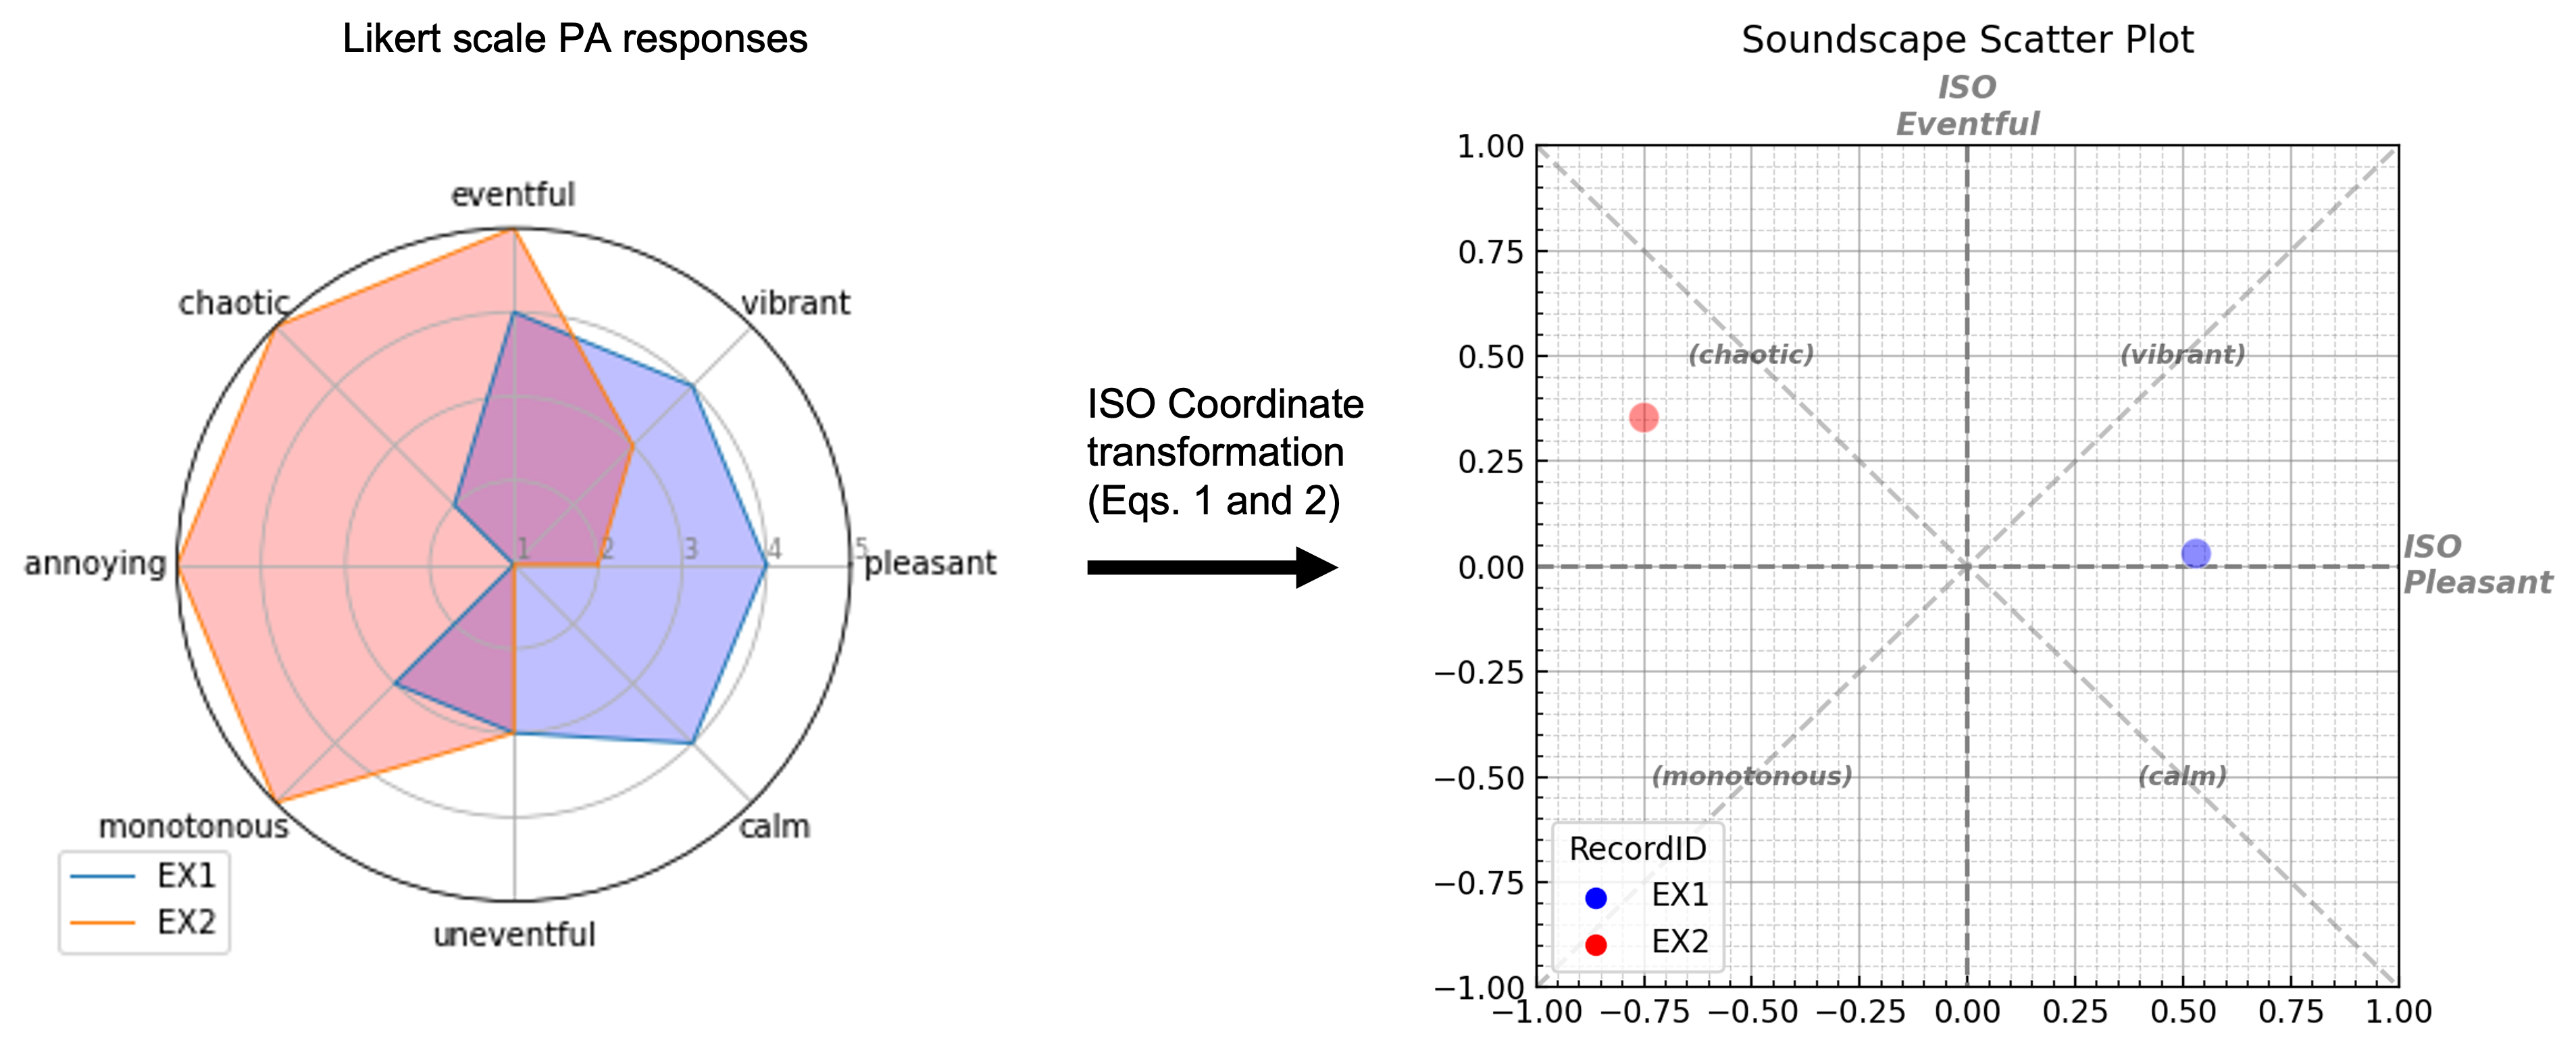
\includegraphics{figures/Figure1.jpg}

}

\caption{\label{fig-radar}Example of representations of two soundscape
assessments. Left: Radar plot of two example perceptual attribute (PA)
ratings on the Likert scales (1 to 5). Right: Scatter plot of the same
assessments on the soundscape circumplex, transformed according to ISO
12913 Part 3.}

\end{figure}

\hypertarget{summarising-the-soundscape-assessment-of-a-location}{%
\subsection{Summarising the soundscape assessment of a
location}\label{summarising-the-soundscape-assessment-of-a-location}}

While the assessment methods available are able to record the soundscape
perception of a single individual, and that person's perception is valid
for themselves, it is not appropriate to then state that it is
representative of the collective perception of that soundscape. In order
to characterise the soundscape of a particular space or time, perceptual
responses from multiple people must be collected and subsequently
summarised or aggregated to describe the general soundscape of the
location. The ISO guidelines stipulate a minimum of 20 participants for
a soundwalk, with these broken up into sessions of no more than 5
participants at a time. Part 3 then provides the recommended methods for
analysing this data.

Annex A.2 of ISO 12913 Part 3 provides the statistical measures to be
used on the raw PA responses. The recommended measure of central
tendency is the median, while the recommended measure of dispersion is
the range. These are chosen as the data is ordinal by nature, however as
will be demonstrated later, they have significant limitations. Although
it is unclear, the implied intention is then that the median value of
each PA is fed into Equation~\ref{eq-pleasant} and
Equation~\ref{eq-eventful} presented above to calculate the ISOPleasant
and ISOEventful values, which can then be plotted in a two-dimensional
scatter plot. Thus the standard suggests that 1) the projection method
equations are not applied to individual responses and 2) only the median
assessment of a location should be plotted.

\hypertarget{limitations-of-the-iso}{%
\subsection{Limitations of the ISO}\label{limitations-of-the-iso}}

How these methods should be applied to represent the soundscape of a
location has not been adequately discussed in previous literature, nor
sufficiently in Part 3 of ISO 1293 itself. Indeed, in Section A.3, the
technical specifications document state that \citep[5]{ISO12913_3}:

\begin{quote}
Results can be reported in a two-dimensional scatter plot with
coordinates for the two dimensions `pleasantness' and `eventfulness'.
The coordinates for `pleasantness' are plotted on the X-axis, and the
coordinates for `eventfulness' on the Y-axis. Every data point in the
scatter plot represents one investigated site.
\end{quote}

However, it is not made clear whether this single point on the
circumplex can be considered to be a realistic representation of the
average perception of the acoustic environment. Effectively, there is no
representation of dispersion in the soundscape assessment, nor a
recommended use of the range that was calculated as part of the analysis
recommend in Section A.2 of Part 3 of the ISO 12913. Absent a suggestion
from the ISO 12913 for how the range should be used, we therefore apply
this analysis to an existing real-world soundscape dataset to determine
whether it provides a useful measure of dispersion. Here we use the data
contained in the International Soundscape Database (ISD)
\citep{Mitchell2021International}, which includes 1,300+ individual
responses collected across 13 locations in London and Venice, according
to the SSID Protocol, which is based on the ISO methods explored in this
paper \citep{Mitchell2020Protocol}.

For any large enough sample for a site, the range will always be from 1
to 5, the maximum and minimum available Likert-scale values. We would
expect that collecting more data would result in more information or
better precision, however the range will always increase as the sample
size increases. As an example, within the ISD data, of the 8 PAs
collected at 13 locations (for a total of 104 scales), 88\% have a range
from 1 to 5 and with larger sample sizes at each location, this
percentage would only have increased. Using range to analyse the
dispersion provides very limited information for comparing the
soundscape assessments of different locations, or of a location under
different conditions.

Although the range does not appear to be a useful measure of dispersion,
the median does provide a useful measure and appropriately functions to
describe the central tendency of the soundscape assessment of the
sample. However, by stipulating that the median of each PA should be
taken prior to applying the circumplex projection, the ISO procedure
only allows for plotting a single scatter point in the circumplex for
each location and does not allow for plotting individual responses on
the circumplex. This limits the possibilities for visualising the
general trends in individual perception across the soundscape. Finally,
no example or recommendation for how the circumplex scatter plot should
be presented is given in the standard.

The instruments described in the ISO 12913 Part 2 \citep{ISO12913_2}
were originally designed primarily for the context of individual or
small group assessments. In these scenarios, the focus is on assessing
the particular soundscape perception of the person in question. Recent
advances in the soundscape approach since the development of the
standards have shifted some focus from individual soundscapes to
characterising the overall soundscape of public spaces
\citep{Mitchell2020Protocol} and to making comparisons between different
groups of people \citep{Jeon2018cross}. In this context, a consideration
of the natural variation in people's perception and the variation over
time of a soundscape must be a core feature of how the soundscape is
discussed. Reducing a public space which may have between tens and tens
of thousands of people moving through it in a single day down to the
mean (or median, or any other single metric) soundscape assessment often
dismisses the reality of the space. Likewise, this overall soundscape of
a public space cannot be determined through a ten person soundwalk, as
there is no guarantee that the sample of people engaged in the soundwalk
is representative of the users of the space (in fact it is likely they
would not be).

\hypertarget{the-way-forward-pleasant-eventful-coordinates-and-probabilistic-soundscape-representation}{%
\section{The Way Forward: Pleasant-Eventful Coordinates and
Probabilistic Soundscape
Representation}\label{the-way-forward-pleasant-eventful-coordinates-and-probabilistic-soundscape-representation}}

Given the identified issues with the recommended methods for statistical
analysis and their shortcomings in representing the variation in
perception of the soundscape in a space, how then should we discuss or
present the results of these soundscape assessments? Ideally, the method
will: 1) take advantage of the circumplex coordinates and their ability
to be displayed on a scatter plot and treated as continuous variables,
2) scale from a dataset of twenty responses to thousands of responses,
3) facilitate the comparison of the soundscapes of different locations,
conditions, and groups, and 4) encapsulate the nuances and diversity of
soundscape perception by representing the distribution of responses.

We therefore present a visualisation in Figure~\ref{fig-circ} of the
soundscape assessments of several urban spaces included in the ISD
\citep{Mitchell2021International} which reflects these goals. The
specific locations selected from the ISD are chosen for demonstration
only and these methods can be applied to any location. Rather than
attempting to represent a single individual's soundscape or of
describing a location's soundscape as a single average assessment (as in
\citet{Mitchell2021Investigating}), this representation shows the whole
range of perception of the users of the space. First, rather than
calculating the median response to each PA in the location, then
calculating the circumplex coordinates, the coordinates for each
individual response are calculated. This results in a vector of
ISOPleasant, ISOEventful values which are continuous variables from -1
to +1 and can be analysed statistically by calculating summary
statistics (mean, standard deviation, quantiles, etc.) and through the
use of regression modelling, which can often be simpler and more
familiar than the recommended methods of analysing ordinal data. This
also enables each individual's response to be placed within the
pleasant-eventful space. All of the responses for a location can then be
plotted, giving an overall scatter plot for a location, as demonstrated
in Figure~\ref{fig-circ-1}.

\begin{figure}

\begin{minipage}[t]{0.47\linewidth}

{\centering 

\raisebox{-\height}{

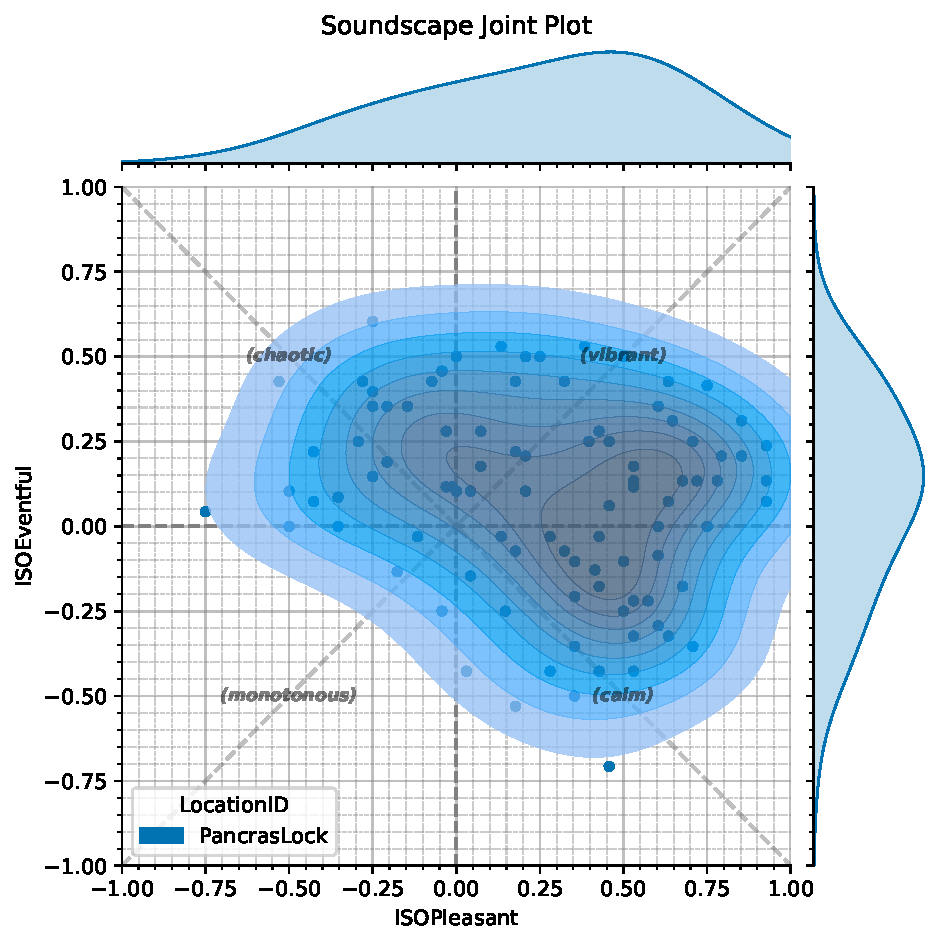
\includegraphics{index_files/figure-pdf/fig-circ-output-1.pdf}

}

}

\subcaption{\label{fig-circ-1}Example distribution of the soundscape
perception of an urban park}
\end{minipage}%
%
\begin{minipage}[t]{0.03\linewidth}

{\centering 

~

}

\end{minipage}%
%
\begin{minipage}[t]{0.50\linewidth}

{\centering 

\raisebox{-\height}{

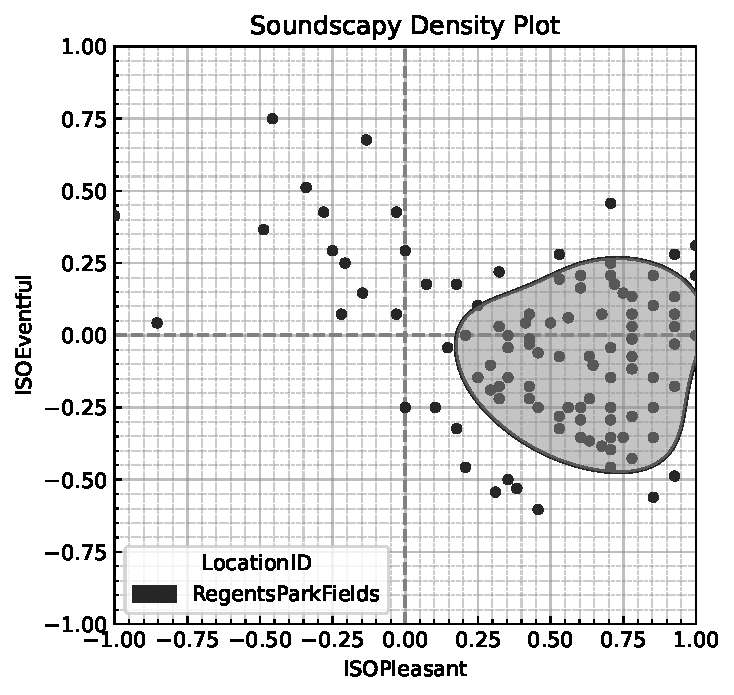
\includegraphics{index_files/figure-pdf/fig-circ-output-2.pdf}

}

}

\subcaption{\label{fig-circ-2}Median perception contour and scatter plot
of individual assessments}
\end{minipage}%
\newline
\begin{minipage}[t]{0.50\linewidth}

{\centering 

\raisebox{-\height}{

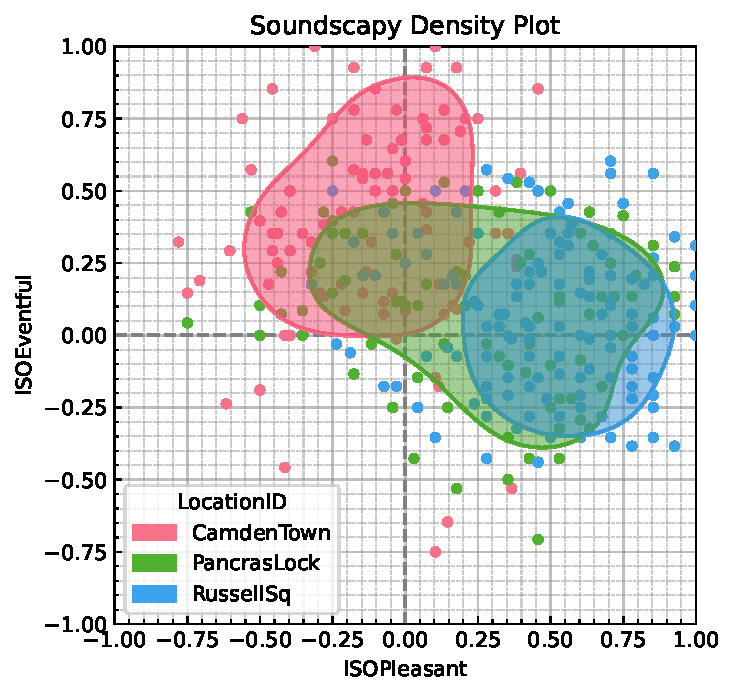
\includegraphics{index_files/figure-pdf/fig-circ-output-3.pdf}

}

}

\subcaption{\label{fig-circ-3}Comparison of the soundscapes of three
urban spaces}
\end{minipage}%
%
\begin{minipage}[t]{0.03\linewidth}

{\centering 

~

}

\end{minipage}%
%
\begin{minipage}[t]{0.47\linewidth}

{\centering 

\raisebox{-\height}{

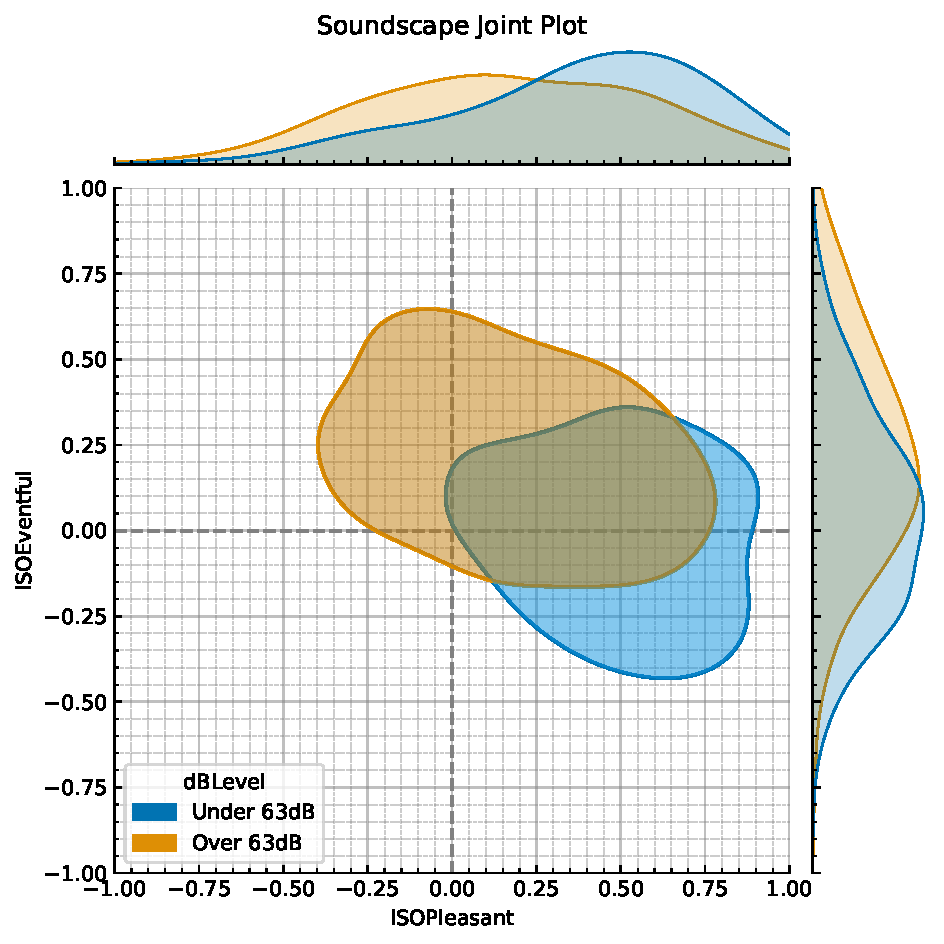
\includegraphics{index_files/figure-pdf/fig-circ-output-4.pdf}

}

}

\subcaption{\label{fig-circ-4}Soundscape perception as a function of
sound level}
\end{minipage}%

\caption{\label{fig-circ}A demonstration of some use cases of
representing soundscape perception as probabilistic distributions. Data
is drawn from the International Soundscape Database (ISD) and is used
for demonstration only. (a) Demonstrates a high level of detail for
presenting the bivariate distribution of soundscape perception in a park
(Russell Square in London). (b) Simplified view of the distribution
using the 50th percentile contour. The assessments impacted by a series
of helicopter fly-overs are made obvious in the chaotic quadrant. (c) A
comparison of three popular public spaces in London. Their overlapping
regions can reveal when and how their soundscapes may be similar. (d) A
comparison across the full ISD for soundscape perception at
\(<65 dB L_{Aeq}\) and \(> 65 dBA\). The introduction of other acoustic,
environmental, and contextual data can reveal new and complex
relationships with the soundscape perception.}

\end{figure}

Once these individual responses are plotted, we then overlay a heatmap
of the bivariate distribution (with isodensity curves for each decile)
and marginal distribution plots\footnote{The specifics of the bivariate
  kernel density estimation \citep{silverman2018density} are beyond the
  scope of this discussion and the most appropriate hyperparameters
  (e.g.~estimation methods, smoothing factors) for this visualisation
  may need to be further explored. These parameters will likely depend
  on the specific dataset used.}. In this way, three primary
characteristics of the soundscape perception can be seen:

\begin{enumerate}
\def\labelenumi{\arabic{enumi}.}
\item
  The distribution across both pleasantness and eventfulness, including
  the central tendency, the dispersion, and any skewness in the
  response;
\item
  The general shape of the soundscape within the space - in this case,
  Russell Sq is almost entirely in the pleasant half but is split
  relatively evenly across the eventfulness space, meaning while it is
  perceived as generally pleasant, it is not strongly calm or vibrant;
\item
  The degree of agreement about the soundscape perception among the
  sample - there appears to be a relatively high agreement about the
  character of Russell Sq, as demonstrated by the compactness of the
  distribution, but this is not the case for every location.
\end{enumerate}

Figure~\ref{fig-circ-1} includes several in-depth visualisations of the
distribution of soundscape assessments, however the detail included can
make further analysis difficult. In particular, a decile heatmap is so
visually busy that, in our experience, it is not possible to plot more
than one soundscape distribution at a time without the figure becoming
overly busy. It also can make it difficult to truly grasp point 2, the
general shape of the soundscape. To facilitate this, the soundscape can
be represented by its 50th percentile contour, as demonstrated in
Figure~\ref{fig-circ-2} where the shaded portion contains 50\% of the
responses. This simplified view of the distribution presents several
advantages, as is demonstrated in Figure~\ref{fig-circ-3} and
Figure~\ref{fig-circ-4} and takes inspiration from the recommendation in
the ISO standard to use the median as a summary statistic. In our
testing, the 50th percentile contour has proved useful, clear, and
compact, however this should not be taken as the definitive correct
percentile cutoff. Further work will need to be done to validate the
precise presentation.

When visualised this way, it is possible to identify outliers and
responses which are the result of anomalous sound events. For instance
if during a survey session at a calm park, a fleet of helicopters flies
overhead, driving the participants to respond that the soundscape is
highly chaotic, we would see a group of scatter points in the chaotic
quadrant which appear obviously outside the general pattern of
responses. Often, these responses would be entirely discarded as
outliers or the surveys and soundwalks would be halted entirely --
ignoring what is in fact a significant impact on that location, its
soundscape, and how useful it may be for the community. Alternatively,
they would be naively included within the statistical analysis,
significantly impacting the central tendency and dispersion metrics
(i.e.~median and range) without consideration for the context. This is
the situation shown in Figure~\ref{fig-circ-2} where it is obvious that
there is strong agreement that Regents Park Fields is highly pleasant
and calm, however we can see numerous responses which assessed it as
highly chaotic. These responses were taken when a series of military
helicopter flyovers drastically changed the sound environment of the
space for several minutes.

Figure~\ref{fig-circ-3} demonstrates how this simplified 50th percentile
contour representation makes it possible to compare the soundscape of
several locations in a sophisticated way. The soundscape assessments of
three urban spaces, Camden Town, Pancras Lock, and Russell Square, are
shown overlaid with each other. We can see that Camden Town, a busy and
crowded street corner with high levels of traffic noise and amplified
music, is generally perceived as chaotic, but the median contour shape
which characterises it also crosses over into the vibrant quadrant. We
can also see that, for a part of the sample, Russell Square and Pancras
Lock are both perceived as similarly pleasant, however some portion of
the responses perceived Pancras Lock as being somewhat chaotic and
annoying. This kind of visualisation can highlight these similarities
between the soundscapes in the locations and identify how they differ.
From here, further investigation could lead us to answer what factors
led to those people perceiving the location as unpleasant, and what
similarities the soundscape of Pancras Lock has with Russell Square that
could perhaps be enhanced to increase the proportion of people
perceiving it as more pleasant.

In addition to solely analysing the distributions of the perceptual
responses themselves, this method can also be combined with other
acoustic, environmental, and contextual data. The final example, in
Figure~\ref{fig-circ-4} demonstrates how this method can better
demonstrate the complex relationships between acoustic features of the
sound environment and the soundscape perception. The data in the ISD
includes \textasciitilde30-s-long binaural audio recordings taken while
each participant was responding to the soundscape survey, providing an
indication of the exact sound environment they were exposed to. For
Figure~\ref{fig-circ-4} the entire dataset of 1,338 responses at all 13
locations has been split according to the analysis of these recordings
giving a set of less than 65 dB \(L_{Aeq}\) and a set of more than 65
dB. The bivariate distributions of these two conditions are then
plotted.

By presenting soundscape perception as a bivariate distributional shape
on the circumplex, practitioners are obligated to address two key
aspects of perception that are too often ignored: the distribution of
potential responses and the eventful dimension. The array of potential
responses to an environment is a crucial factor in assessing the
successful design of a space and represents the reality of perception.
There is no single perceptual outcome of an environment; it will always
include some randomness inherent in human perception and this should be
reflected in how we present soundscape assessments. Similarly, the
eventful dimension is crucial to understanding how an environment is
perceived and can have important impacts on the health and well-being of
the users. Recent evidence also suggests that there is a more direct
relationship between acoustic characteristics and the perception of
eventfulness, while pleasantness is more dependent on context
\citep{Mitchell2021Investigating}. Studies that explore the correlations
between acoustic features and annoyance (or pleasantness) without
considering eventfulness are perhaps missing the most direct effect of
the acoustic features.

\hypertarget{making-use-of-the-soundscape-circumplex}{%
\section{Making Use of the Soundscape
Circumplex}\label{making-use-of-the-soundscape-circumplex}}

There are various potential methods for integrating the probabilistic
soundscape approach into a design and intervention setting. Representing
the soundscape as a shape within the circumplex provides flexibility in
setting design goals for a space. Not all spaces can or should have the
same soundscape and soundscapes should be treated as dynamic, not
static; identifying and creating an appropriate soundscape for the
particular use case of a space is crucial to guiding its design. Proper
forward-looking design of a soundscape would involve defining the
desired shape and distribution of perceptions in the space. This can be
achieved by drawing the desired shape in the circumplex and testing
interventions which will bring the existing soundscape closer to the
desired perception. A soundscape may need to be perceived as vibrant
during the day and calm for some portion of the evening, meaning the
desired shape should primarily sit within the vibrant quadrant but have
some overlap into calm. This also enables designers to recognise the
limitations of their environment and acknowledge that it is not always
possible to transform a highly chaotic soundscape into a calm one. In
these cases, instead the focus should be placed on shifting the
distribution to some degree in a positive direction. The most
sophisticated method of setting design goals is therefore to identify
the desired shape which represents the variety of desired outcomes, and
focus on designs and interventions which are most successful in matching
the predicted outcome with that goal.

Although the visualisations shown in Figure~\ref{fig-circ} are a
powerful tool for viewing, analysing, and discussing the
multi-dimensional aspects of soundscape perception, there are certainly
cases where simpler metrics are needed to aid discussion and to set
design goals. For this, the underlying process of calculating the
ISOPleasant and ISOEventful coordinates for each individual response is
still the first step in analysing the quantitative soundscape data.
These sets of coordinates can then be analysed and summarised in various
ways. One approach which takes inspiration from noise annoyance
\citep{ISO15666}, is to discuss the ``percent of people likely to
perceive'' a soundscape as pleasant, vibrant, etc. when it is necessary
to use numerical descriptions. In this way, a numerical design goal
could also be set as e.g.~`the soundscape should be likely to be
perceived as pleasant by at least 75\% of users' or the result of an
intervention presented as e.g.~`the likelihood of the soundscape being
perceived as calm increased from 30\% to 55\%'. These numbers can be
drawn from either actual surveys or from the results of predictive
models.

Although acknowledging the distribution of responses is crucial, it is
sometimes necessary to summarise locations down to a single point to
compare many different locations and to easily investigate how the
soundscape assessment has generally changed over time. For this purpose,
the mean of the ISOPleasant and ISOEventful values across all
respondents is calculated to result in a single coordinate point per
location. This clearly mirrors the original intent of the coordinate
transformation presented in the ISO, but by applying the transformation
first to each individual assessment then calculating the mean value, it
maintains a direct link to the distributions shown in
Figure~\ref{fig-circ}. An example plot using the mean response of each
location to compare many locations and to demonstrate change in
soundscape perception can be found in Figure 5 of
\citet{Mitchell2021Investigating}. The key to all of these analysis
methods, whether they be the distributional plots shown in
Figure~\ref{fig-circ}, the numerical summaries, or the use of other
standard statistical analyses is treating the soundscape of the space or
group as a collective perception as expressed by a vector of individual
circumplex coordinates.

Finally, the primary concern addressed by this method is the analysis of
larger soundscape datasets, compared to what is suggested in the
standard. This is necessary in order to statistically describe the
groups or sub-groups being investigated, and is typically taken to need
a minimum of \textasciitilde30 responses per group (although the full
dataset, made up of many groups and locations may have many more
responses in total, as in the ISD)
\citep[e.g.][]{Hong2015Influence, PuyanaRomero2016Modelling}. It is
unlikely that the bivariate distributions plots shown are appropriate
for small datasets. However, the process of calculating the ISO
coordinates for each individual response and treating this as a set of
continuous values to subject to other statistical analysis holds for all
sample sizes. Pleasant-eventful scatterplots are still useful for
comparing differences in individual responses and appropriate methods of
summarising small sample data should be explored (such as the univariate
scatterplots described in \citet{Weissgerber2015Bar}).

\hypertarget{limitations-of-the-circumplex-and-quantitative-analysis}{%
\subsection{Limitations of the circumplex and quantitative
analysis}\label{limitations-of-the-circumplex-and-quantitative-analysis}}

The method presented here is a solution for representing the soundscape
of a space, which requires considering the perception of many people,
but it is important to note that this is only one (very important) goal
of the soundscape approach. Psychological and sociological
investigations of people's relationship to their sound environment and
the interactions between social contexts and individual perception are a
crucial aspect of the field for which this approach would likely not be
sufficient \citep{Bild2018Public}. Open-response questions, structured
interviews, and mixed-methods studies can provide additional insight
into how people experience their environment and should be considered
alongside or preceding this focus on how a space is likely to be
perceived on a larger scale.

These other approaches are not in opposition to the methods proposed
here, but instead further expand our view. The circumplex is a limited
view of soundscape perception (this is made obvious by the fact that it
excludes the third component, \emph{familiarity}, identified in
\citet{Axelsson2010Principal}) but it is an exceptionally rich tool for
dealing with the two primary aspects of soundscape perception which can
readily expand the much more limited view provided by existing noise and
annoyance assessment tools. Aspects of the psychological and
sociological emphasis can also be integrated into a circumplex-focused
approach, as demonstrated in \citet{Erfanian2021Psychological}, where
personal factors such as age, gender, and psychological well-being were
analysed in terms of how they mediated the ISOPleasant and ISOEventful
outcomes.

There has been some discussion regarding the interdependence of the PAs
and the strict validity of the 90\degree and 45 \degree relationships
between the attributes \citep{Lionello2021Introducing}. Further work has
indicated that the scaling between the attributes may vary, but the
underlying relationships hold. It is for this reason that we have taken
the coordinate projection as the starting point of this critique. It
should also be noted that the particular PA descriptors used in ISO
12913 are intended for outdoor environments and should not be directly
applied to indoor spaces. However, a proposed set of descriptors for
some indoor environments has been derived which further confirms the
validity of the circumplex relationships \citep{Torresin2020Indoor}. The
methods proposed here should be directly applicable to indoor spaces by
using the comfort/content descriptors as well as to any other
translations of soundscape descriptors into other languages
\citep{Aletta2020Soundscape} as long as the dimensional relationships of
the circumplex are maintained.

\hypertarget{conclusions}{%
\section{Conclusions}\label{conclusions}}

Soundscape studies have been steadily growing as a research field over
the past three decades. Their relevance for the planning and design of
urban spaces is now generally acknowledged by both the academic and
practitioners' communities. Yet, for their contribution in shaping
better environments to be meaningful, it is necessary to agree on common
methodological approaches and techniques to analyse and present
standardised soundscape data. Therefore, the general goal of this work
is to consider some of the questions that may still have been left
unanswered by the ISO 12913 series when it comes to optimal ways to
analyse and represent soundscape data coming from the ISO standardised
protocols. As a result, we propose a method for presenting the results
of standardised assessments as a distribution of soundscape perception
within the circumplex space. This method provides an opportunity to
conduct a nuanced discussion of soundscape perception which considers
the variety of individual responses. The tools for generating these
circumplex visualisations are made openly available as well. This shift
is part of a move towards a more holistic approach to urban noise and to
integrating the soundscape approach into urban design and regulations.

\hypertarget{data-and-code-availability}{%
\section{Data and Code Availability}\label{data-and-code-availability}}

The data used in this study are openly available as v0.2.3 of the
International Soundscape Database (ISD) at
\url{https://zenodo.org/record/5578572}. A library of python functions
for producing the type of plots presented (using the seaborn plotting
library \citep{Waskom2021}) and an interactive Jupyter notebook which
provides a tutorial for using this code, working with the ISD data, and
recreating the figures of this paper has been made available as part of
the ISD.

\hypertarget{acknowledgements}{%
\section{Acknowledgements}\label{acknowledgements}}

This project has received funding from the European Research Council
(ERC) under the European Union's Horizon 2020 research and innovation
program (grant agreement No.~740696, project title: Soundscape Indices -
SSID). We would like to acknowledge Matteo Lionello for the helpful
discussions, and (in alphabetical order) Mercede Erfanian, Magdalena
Kachlicka, and Tin Oberman for the helpful discussions and the data
collection support.


  \bibliography{references.bib}


\end{document}
